% answers.tex —— 2012 年·全国新课标卷·理科 · 参考答案与详细解析片段
% 由 tools/generate_projects.py 依来源总账自 2012/2012_数学真题_全国新课标理_试题.md + 2012/2012_数学真题_全国新课标理_解析正文.md + 2012/2012_数学真题_全国新课标理_答案要点.md 生成，勿手改（改源 MD 后重跑）


\begin{answer}
\gksolhead{1}{}

\textbf{题目}：

已知集合 $A=\{1,2,3,4,5\}$，$B=\{(x,y)\mid x\in A,\ y\in A,\ x-y\in A\}$，则 $B$ 中所含元素的个数为\mbox{（　　）}

（A）$3$　（B）$6$　（C）$8$　（D）$10$

\Needspace{4\baselineskip}
\textbf{解析}

要使 $(x,y)\in B$，必须有 $x-y\in\{1,2,3,4,5\}$，即 $x>y$。在 $1,2,3,4,5$ 中，差为 $1,2,3,4$ 的有 $4,3,2,1$ 对，故共有 $10$ 个，选 D。

\gkanswer{答案：D}

\end{answer}
\begin{answer}
\gksolhead{2}{}

\textbf{题目}：

将 $2$ 名教师、$4$ 名学生分成 $2$ 个小组，分别安排到甲、乙两地参加社会实践活动，每个小组由 $1$ 名教师和 $2$ 名学生组成，不同的安排方案共有\mbox{（　　）}

（A）$12$ 种　（B）$10$ 种　（C）$9$ 种　（D）$8$ 种

\Needspace{4\baselineskip}
\textbf{解析}

先把两名教师分别安排到甲、乙两地，有 $2$ 种方法；再从四名学生中选两名到甲地，剩下两名到乙地，有 $\binom42=6$ 种方法。因此共有 $2\binom42=12$ 种，选 A。

\gkanswer{答案：A}

\end{answer}
\begin{answer}
\gksolhead{3}{}

\textbf{题目}：

下面是关于复数 $z=\dfrac{2}{-1+i}$ 的四个命题：

$p_1$：$|z|=2$；$p_2$：$z^2=2i$；$p_3$：$z$ 的共轭复数为 $1+i$；$p_4$：$z$ 的虚部为 $-1$。其中的真命题为\mbox{（　　）}

（A）$p_2,p_3$　（B）$p_1,p_2$　（C）$p_2,p_4$　（D）$p_3,p_4$

\Needspace{4\baselineskip}
\textbf{解析}

\nopagebreak[4]
\[
z=\frac{2}{-1+i}=\frac{2(-1-i)}{(-1+i)(-1-i)}=-1-i.
\]
所以 $|z|=\sqrt2\ne2$，$z^2=2i$，$\overline z=-1+i\ne1+i$，且 $z$ 的虚部为 $-1$。真命题为 $p_2,p_4$，选 C。

\gkanswer{答案：C}

\end{answer}
\begin{answer}
\gksolhead{4}{}

\textbf{题目}：

设 $F_1,F_2$ 是椭圆 $E:\dfrac{x^2}{a^2}+\dfrac{y^2}{b^2}=1$（$a>b>0$）的左、右焦点，$P$ 为直线 $x=\dfrac{3a}{2}$ 上一点，$\triangle F_2PF_1$ 是底角为 $30^\circ$ 的等腰三角形，则 $E$ 的离心率为\mbox{（　　）}

（A）$\dfrac12$　（B）$\dfrac23$　（C）$\dfrac34$　（D）$\dfrac45$

\Needspace{4\baselineskip}
\textbf{解析}

\Needspace{5\baselineskip}
设椭圆焦半距为 $c$，取 $P$ 在上方。由等腰三角形的两个底角均为 $30^\circ$，可取底边为 $PF_1$，于是
\nopagebreak[4]
\[
PF_2=F_1F_2=2c,\qquad
\tan30^\circ=\frac{y_P}{\frac32a+c}.
\]
\Needspace{5\baselineskip}
故 $y_P=(\frac32a+c)/\sqrt3$。再由 $PF_2=2c$，
\nopagebreak[4]
\[
\left(\frac32a-c\right)^2+\frac{(\frac32a+c)^2}{3}=4c^2.
\]
\Needspace{5\baselineskip}
化简得 $\frac32a=2c$，所以离心率
\nopagebreak[4]
\[
e=\frac ca=\frac34,
\]
选 C。

\gkanswer{答案：C}

\end{answer}
\begin{answer}
\gksolhead{5}{}

\textbf{题目}：

已知 $\{a_n\}$ 为等比数列，$a_4+a_7=2$，$a_5a_6=-8$，则 $a_1+a_{10}=$\mbox{（　　）}

（A）$7$　（B）$5$　（C）$-5$　（D）$-7$

\Needspace{4\baselineskip}
\textbf{解析}

\Needspace{5\baselineskip}
令 $r=q^3$，则 $a_4(1+r)=2$，且 $a_5a_6=a_4^2r=-8$。消去 $a_4$ 得
\nopagebreak[4]
\[
\frac{4r}{(1+r)^2}=-8,\qquad
2r^2+5r+2=0,
\]
\Needspace{5\baselineskip}
所以 $r=-\frac12$ 或 $r=-2$。又
\nopagebreak[4]
\[
a_1+a_{10}=a_4\left(\frac1r+r^2\right).
\]
分别代入两种 $r$，均得 $a_1+a_{10}=-7$，选 D。

\gkanswer{答案：D}

\end{answer}
\begin{answer}
\gksolhead{6}{}

\textbf{题目}：

如果执行下面的程序框图，输入正整数 $N$（$N\geqslant2$）和实数 $a_1,a_2,\cdots,a_N$，输出 $A,B$，则\mbox{（　　）}
\nopagebreak[4]
\begin{center}\begin{tikzpicture}[
  >=stealth,
  node distance=7mm and 12mm,
  every node/.style={font=\small},
  scale=.78,
  transform shape
]
\node[draw,rounded corners,minimum width=18mm,minimum height=7mm] (start) {开始};
\node[draw,trapezium,trapezium left angle=75,trapezium right angle=105,
      minimum width=43mm,minimum height=7mm,below=of start]
      (input) {输入 $N,a_1,a_2,\ldots,a_N$};
\node[draw,minimum width=38mm,minimum height=7mm,below=of input]
      (init) {$k=1,\ A=a_1,\ B=a_1$};
\node[draw,minimum width=20mm,minimum height=7mm,below=of init]
      (read) {$x=a_k$};
\node[draw,diamond,aspect=2.2,below=of read,minimum width=25mm,minimum height=8mm]
      (max) {$x>A$};
\node[draw,minimum width=18mm,minimum height=7mm,right=of max]
      (setmax) {$A=x$};
\node[draw,diamond,aspect=2.2,below=of max,minimum width=25mm,minimum height=8mm]
      (min) {$x<B$};
\node[draw,minimum width=18mm,minimum height=7mm,left=of min]
      (setmin) {$B=x$};
\node[draw,diamond,aspect=2.2,below=of min,minimum width=25mm,minimum height=8mm]
      (done) {$k\geqslant N$};
\node[draw,minimum width=25mm,minimum height=7mm,right=of done]
      (inc) {$k=k+1$};
\node[draw,trapezium,trapezium left angle=75,trapezium right angle=105,
      minimum width=25mm,minimum height=7mm,below=of done]
      (out) {输出 $A,B$};
\node[draw,rounded corners,minimum width=18mm,minimum height=7mm,below=of out]
      (end) {结束};

\draw[->] (start)--(input)--(init)--(read)--(max);
\draw[->] (max)--node[above]{是}(setmax)--++(0,-.65) |- (done);
\draw[->] (max)--node[right]{否}(min);
\draw[->] (min)--node[above]{是}(setmin)--++(0,-.65) |- (done);
\draw[->] (min)--node[right]{否}(done);
\draw[->] (done)--node[above]{否}(inc) |- (read);
\draw[->] (done)--node[right]{是}(out)--(end);
\end{tikzpicture}
\end{center}
\nopagebreak[4]
（A）$A+B$ 为 $a_1,a_2,\cdots,a_N$ 的和

（B）$\dfrac{A+B}{2}$ 为 $a_1,a_2,\cdots,a_N$ 的算术平均数

（C）$A$ 和 $B$ 分别是 $a_1,a_2,\cdots,a_N$ 中最大的数和最小的数

（D）$A$ 和 $B$ 分别是 $a_1,a_2,\cdots,a_N$ 中最小的数和最大的数

\Needspace{4\baselineskip}
\textbf{解析}

程序开始令 $A=B=a_1$，随后逐项读取 $a_k$。若 $a_k>A$ 就更新 $A$，若 $a_k<B$ 就更新 $B$，遍历结束时 $A$ 是所有输入数中的最大值，$B$ 是最小值，选 C。

\gkanswer{答案：C}

\end{answer}
\begin{answer}
\gksolhead{7}{}

\textbf{题目}：

如图，网格上小正方形的边长为 $1$，粗线画出的是某几何体的三视图，则此几何体的体积为\mbox{（　　）}
\nopagebreak[4]
\begin{center}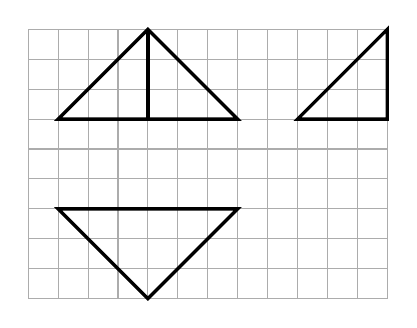
\begin{tikzpicture}[scale=.38]
  \draw[gray!65] (0,0) grid (12,9);
  \draw[very thick] (1,6)--(7,6)--(4,9)--cycle;
  \draw[very thick] (4,6)--(4,9);
  \draw[very thick] (9,6)--(12,6)--(12,9)--cycle;
  \draw[very thick] (1,3)--(7,3)--(4,0)--cycle;
\end{tikzpicture}
\end{center}
\nopagebreak[4]
\begin{gktip}
\textbf{第 7 题图形转录}：固定源印刷页 755 的网格图含三个粗线视图：左上为底边长 $6$、高 $3$ 且标出中线的等腰三角形；右上为两直角边长均为 $3$ 的直角三角形；左下为底边长 $6$、高 $3$ 的倒置等腰三角形。
\end{gktip}

（A）$6$　（B）$9$　（C）$12$　（D）$18$

\Needspace{4\baselineskip}
\textbf{解析}

\Needspace{5\baselineskip}
由三视图可知，该几何体为底面是直角三角形、两直角边均为 $3$、高为 $6$ 的三棱锥。因此
\nopagebreak[4]
\[
V=\frac13\cdot\frac12\cdot3\cdot3\cdot6=9,
\]
选 B。

\gkanswer{答案：B}

\end{answer}
\begin{answer}
\gksolhead{8}{}

\textbf{题目}：

等轴双曲线 $C$ 的中心在原点，焦点在 $x$ 轴上，$C$ 与抛物线 $y^2=16x$ 的准线交于 $A,B$ 两点，$|AB|=4\sqrt3$，则 $C$ 的实轴长为\mbox{（　　）}

（A）$\sqrt2$　（B）$2\sqrt2$　（C）$4$　（D）$8$

\Needspace{4\baselineskip}
\textbf{解析}

\Needspace{5\baselineskip}
等轴双曲线可设为
\nopagebreak[4]
\[
\frac{x^2}{a^2}-\frac{y^2}{a^2}=1.
\]
\Needspace{5\baselineskip}
抛物线 $y^2=16x$ 的准线为 $x=-4$。代入两个交点的纵坐标 $y=\pm2\sqrt3$，得
\nopagebreak[4]
\[
\frac{16-12}{a^2}=1,
\]
即 $a=2$。双曲线的实轴长为 $2a=4$，选 C。

\gkanswer{答案：C}

\end{answer}
\begin{answer}
\gksolhead{9}{}

\textbf{题目}：

已知 $\omega>0$，函数 $f(x)=\sin\left(\omega x+\dfrac{\pi}{4}\right)$ 在 $\left(\dfrac{\pi}{2},\pi\right)$ 单调递减，则 $\omega$ 的取值范围是\mbox{（　　）}

（A）$\left[\dfrac12,\dfrac54\right]$　（B）$\left[\dfrac12,\dfrac34\right]$　（C）$\left(0,\dfrac12\right]$　（D）$(0,2]$

\Needspace{4\baselineskip}
\textbf{解析}

\nopagebreak[4]
\[
f'(x)=\omega\cos\left(\omega x+\frac{\pi}{4}\right).
\]
\Needspace{5\baselineskip}
在 $\left(\frac\pi2,\pi\right)$ 上单调递减时，相位区间必须落在余弦函数的一个负值区间内。由于 $\omega>0$ 且相位从 $\frac\pi4$ 以上开始，只能落在
\nopagebreak[4]
\[
\left[\frac\pi2,\frac{3\pi}2\right]
\]
\Needspace{5\baselineskip}
内，故
\nopagebreak[4]
\[
\frac{\pi}{2}\leqslant\frac{\omega\pi}{2}+\frac\pi4,\qquad
\omega\pi+\frac\pi4\leqslant\frac{3\pi}{2}.
\]
这给出 $\frac12\leqslant\omega\leqslant\frac54$，选 A。

\gkanswer{答案：A}

\end{answer}
\begin{answer}
\gksolhead{10}{}

\textbf{题目}：

已知函数 $f(x)=\dfrac{1}{\ln(x+1)-x}$，则 $y=f(x)$ 的图象大致为\mbox{（　　）}
\nopagebreak[4]
\begin{center}\begin{tikzpicture}[font=\small, x=1.05cm, y=.62cm]
  \begin{scope}
    \draw[->] (-1.25,0)--(2.65,0) node[right] {$x$};
    \draw[->] (0,-4)--(0,3.9) node[above] {$y$};
    \draw (1,-.08)--(1,.08) node[below right,inner sep=1pt] {$1$};
    \draw (-.08,1)--(.08,1) node[left,inner sep=1pt] {$1$};
    \node[below left,inner sep=1pt] at (0,0) {$O$};
    \draw[thick] (.12,3.7) .. controls (.18,2.0) and (.45,.65) .. (2.35,.15);
    \node[below] at (.65,-4.55) {(A)};
  \end{scope}
  \begin{scope}[xshift=5.1cm]
    \draw[->] (-1.25,0)--(2.65,0) node[right] {$x$};
    \draw[->] (0,-4)--(0,3.9) node[above] {$y$};
    \draw (1,-.08)--(1,.08) node[below right,inner sep=1pt] {$1$};
    \draw (-.08,1)--(.08,1) node[left,inner sep=1pt] {$1$};
    \node[below left,inner sep=1pt] at (0,0) {$O$};
    \draw[thick] (-1.05,-.10) .. controls (-.55,-.18) and (-.13,-1.2) .. (-.06,-3.8);
    \draw[thick] (.06,-3.8) .. controls (.13,-1.2) and (.55,-.18) .. (2.35,-.10);
    \node[below] at (.65,-4.55) {(B)};
  \end{scope}
  \begin{scope}[yshift=-5.25cm]
    \draw[->] (-1.25,0)--(2.65,0) node[right] {$x$};
    \draw[->] (0,-4)--(0,3.9) node[above] {$y$};
    \draw (1,-.08)--(1,.08) node[below right,inner sep=1pt] {$1$};
    \draw (-.08,1)--(.08,1) node[left,inner sep=1pt] {$1$};
    \node[below left,inner sep=1pt] at (0,0) {$O$};
    \draw[thick] (-1.05,.10) .. controls (-.55,.18) and (-.13,1.2) .. (-.06,3.8);
    \draw[thick] (.06,-3.8) .. controls (.13,-1.2) and (.55,-.18) .. (2.35,-.10);
    \node[below] at (.65,-4.55) {(C)};
  \end{scope}
  \begin{scope}[xshift=5.1cm,yshift=-5.25cm]
    \draw[->] (-1.25,0)--(2.65,0) node[right] {$x$};
    \draw[->] (0,-4)--(0,3.9) node[above] {$y$};
    \draw (1,-.08)--(1,.08) node[below right,inner sep=1pt] {$1$};
    \draw (-.08,1)--(.08,1) node[left,inner sep=1pt] {$1$};
    \node[below left,inner sep=1pt] at (0,0) {$O$};
    \draw[thick] (.06,-3.8) .. controls (.13,-1.2) and (.55,-.18) .. (2.35,-.10);
    \node[below] at (.65,-4.55) {(D)};
  \end{scope}
\end{tikzpicture}
\end{center}
\nopagebreak[4]
（A）图 A　（B）图 B　（C）图 C　（D）图 D

\Needspace{4\baselineskip}
\textbf{解析}

\Needspace{5\baselineskip}
定义域为 $x>-1$ 且 $x\ne0$。由 $\ln(1+x)<x$（$x>-1$ 且 $x\ne0$），有
\nopagebreak[4]
\[
\ln(1+x)-x<0.
\]
因此函数在 $(-1,0)$ 和 $(0,+\infty)$ 上均为负值；且 $x\to0^\pm$ 时分母趋于 $0-$，函数趋于 $-\infty$，$x\to-1^+$ 或 $x\to+\infty$ 时函数趋于 $0-$。图象应为左右两支均在 $x$ 轴下方、以 $x=0$ 为竖直渐近线的图形，选 B。

\gkanswer{答案：B}

\end{answer}
\begin{answer}
\gksolhead{11}{}

\textbf{题目}：

已知三棱锥 $S-ABC$ 的所有顶点都在球 $O$ 的球面上，$\triangle ABC$ 是边长为 $1$ 的正三角形，$SC$ 为球 $O$ 的直径，且 $SC=2$，则此棱锥的体积为\mbox{（　　）}

（A）$\dfrac{\sqrt2}{6}$　（B）$\dfrac{\sqrt3}{6}$　（C）$\dfrac{\sqrt2}{3}$　（D）$\dfrac{\sqrt2}{2}$

\Needspace{4\baselineskip}
\textbf{解析}

\Needspace{5\baselineskip}
取 $C=(0,0,0)$，令 $A=(1,0,0)$、$B=(\frac12,\frac{\sqrt3}{2},0)$。因为 $SC$ 是直径，$\angle SAC=\angle SBC=90^\circ$，从而 $SA=SB=\sqrt3$。设 $S=(u,v,w)$，由 $SC=2$、$SA=SB=\sqrt3$ 可得
\nopagebreak[4]
\[
S=\left(1,\frac1{\sqrt3},\pm2\sqrt{\frac23}\right).
\]
\Needspace{5\baselineskip}
所以三棱锥的高为 $2\sqrt{\frac23}$，底面面积为 $\frac{\sqrt3}{4}$，体积为
\nopagebreak[4]
\[
V=\frac13\cdot\frac{\sqrt3}{4}\cdot2\sqrt{\frac23}
=\frac{\sqrt2}{6},
\]
选 A。

\gkanswer{答案：A}

\end{answer}
\begin{answer}
\gksolhead{12}{}

\textbf{题目}：

设点 $P$ 在曲线 $y=\dfrac12\mathrm e^x$ 上，点 $Q$ 在曲线 $y=\ln(2x)$ 上，则 $|PQ|$ 的最小值为\mbox{（　　）}

（A）$1-\ln2$　（B）$\sqrt2(1-\ln2)$　（C）$1+\ln2$　（D）$\sqrt2(1+\ln2)$

\Needspace{4\baselineskip}
\textbf{解析}

\Needspace{5\baselineskip}
曲线 $y=\ln(2x)$ 是曲线 $y=\frac12\mathrm e^x$ 关于直线 $y=x$ 的对称曲线。对 $y=\frac12\mathrm e^x$，有
\nopagebreak[4]
\[
y-x=\frac12\mathrm e^x-x.
\]
\Needspace{5\baselineskip}
其最小值在 $x=\ln2$ 处取得，值为 $1-\ln2>0$。两条互为关于 $y=x$ 对称的曲线的最短连线垂直于 $y=x$，取对称点
\nopagebreak[4]
\[
P=(\ln2,1),\qquad Q=(1,\ln2),
\]
\Needspace{5\baselineskip}
故
\nopagebreak[4]
\[
|PQ|=\sqrt2(1-\ln2),
\]
选 B。

\gkanswer{答案：B}

\end{answer}
\begin{answer}
\gksolhead{13}{}

\textbf{题目}：

已知向量 $\boldsymbol a,\boldsymbol b$ 夹角为 $45^\circ$，且 $|\boldsymbol a|=1$，$|2\boldsymbol a-\boldsymbol b|=\sqrt{10}$，则 $|\boldsymbol b|=$\gkblank{}。

\Needspace{4\baselineskip}
\textbf{解析}

\Needspace{5\baselineskip}
设 $|\boldsymbol b|=t$。由夹角公式，
\nopagebreak[4]
\[
10=|2\boldsymbol a-\boldsymbol b|^2
=4+t^2-4t\cos45^\circ
=t^2-2\sqrt2t+4.
\]
\Needspace{5\baselineskip}
所以 $t^2-2\sqrt2t-6=0$，取正根得
\nopagebreak[4]
\[
|\boldsymbol b|=3\sqrt2.
\]

\gkanswer{答案：$3\sqrt2$}

\end{answer}
\begin{answer}
\gksolhead{14}{}

\textbf{题目}：

\Needspace{5\baselineskip}
设 $x,y$ 满足约束条件

\nopagebreak[4]
\[
\begin{cases}
x-y\geqslant-1,\\
x+y\leqslant3,\\
x\geqslant0,\\
y\geqslant0,
\end{cases}
\]

则 $z=x-2y$ 的取值范围为\gkblank{}。

\Needspace{4\baselineskip}
\textbf{解析}

\Needspace{5\baselineskip}
可行域的顶点为 $(0,0),(0,1),(1,2),(3,0)$。在这些点上分别有
\nopagebreak[4]
\[
z=0,-2,-3,3,
\]
故取值范围为 $[-3,3]$。

\gkanswer{答案：$[-3,3]$}

\end{answer}
\begin{answer}
\gksolhead{15}{}

\textbf{题目}：

某一部件由三个电子元件按下图方式连接而成，元件 $1$ 或元件 $2$ 正常工作，且元件 $3$ 正常工作，则部件正常工作。设三个电子元件的使用寿命（单位：小时）均服从正态分布 $N(1000,50^2)$，且各个元件能否正常工作相互独立，那么该部件的使用寿命超过 $1000$ 小时的概率为\gkblank{}。
\nopagebreak[4]
\begin{center}\begin{tikzpicture}[font=\small]
  \draw (-.6,0) -- (.55,0);
  \draw (.55,0) -- (.55,1.05) -- (1.15,1.05);
  \draw (.55,0) -- (.55,-1.05) -- (1.15,-1.05);
  \draw (2.65,1.05) -- (3.25,1.05) -- (3.25,0) -- (3.85,0);
  \draw (2.65,-1.05) -- (3.25,-1.05) -- (3.25,0);
  \node[draw,minimum width=1.5cm,minimum height=.62cm] at (1.9,1.05) {元件 1};
  \node[draw,minimum width=1.5cm,minimum height=.62cm] at (1.9,-1.05) {元件 2};
  \node[draw,minimum width=1.5cm,minimum height=.62cm] at (4.6,0) {元件 3};
\end{tikzpicture}
\end{center}
\nopagebreak[4]
\Needspace{4\baselineskip}
\textbf{解析}

\Needspace{5\baselineskip}
由 $N(1000,50^2)$ 的对称性，每个元件的使用寿命超过 $1000$ 小时的概率均为 $\frac12$。元件 $1$ 或元件 $2$ 正常工作的概率为
\nopagebreak[4]
\[
1-\left(\frac12\right)^2=\frac34.
\]
\Needspace{5\baselineskip}
再与元件 $3$ 正常工作的事件相乘，所求概率为
\nopagebreak[4]
\[
\frac34\cdot\frac12=\frac38.
\]

\gkanswer{答案：$\dfrac38$}

\end{answer}
\begin{answer}
\gksolhead{16}{}

\textbf{题目}：

数列 $\{a_n\}$ 满足 $a_{n+1}+(-1)^n a_n=2n-1$，则 $\{a_n\}$ 的前 $60$ 项和为\gkblank{}。

\Needspace{4\baselineskip}
\textbf{解析}

\Needspace{5\baselineskip}
由递推式分别取奇、偶下标，得
\nopagebreak[4]
\[
a_{2k}-a_{2k-1}=4k-3,\qquad
a_{2k+1}+a_{2k}=4k-1.
\]
\Needspace{5\baselineskip}
消去 $a_{2k}$ 得
\nopagebreak[4]
\[
a_{2k+1}=2-a_{2k-1}.
\]
\Needspace{5\baselineskip}
所以奇数项交替为 $a_1,2-a_1$。前 $60$ 项中奇数项之和为 $30$，偶数项之和为
\nopagebreak[4]
\[
30+\sum_{k=1}^{30}(4k-3)=30+1770=1800,
\]
总和为 $30+1800=1830$。

\gkanswer{答案：$1830$}

\end{answer}
\begin{answer}
\gksolhead{17}{}

\textbf{题目}：

已知 $a,b,c$ 分别为 $\triangle ABC$ 三个内角 $A,B,C$ 的对边，$a\cos C+\sqrt3a\sin C-b-c=0$。

（1） 求 $A$；

（2） 若 $a=2$，$\triangle ABC$ 的面积为 $\sqrt3$，求 $b,c$。

\Needspace{4\baselineskip}
\textbf{解析}

\gksubpart{(1) 解}

\Needspace{5\baselineskip}
由正弦定理，原式除以 $2R$ 后化为
\nopagebreak[4]
\[
\sin A\cos C+\sqrt3\sin A\sin C-\sin B-\sin C=0.
\]
\Needspace{5\baselineskip}
利用 $B=\pi-A-C$，有
\nopagebreak[4]
\[
\sin B+\sin C=\sin(A+C)+\sin C
=\sin A\cos C+(\cos A+1)\sin C.
\]
\Needspace{5\baselineskip}
约去 $\sin C>0$，得到
\nopagebreak[4]
\[
\sqrt3\sin A=1+\cos A.
\]
即 $\tan\frac A2=\frac1{\sqrt3}$，所以 $A=60^\circ$。

\gksubpart{(2) 解}

\Needspace{5\baselineskip}
面积条件给出
\nopagebreak[4]
\[
\frac12bc\sin60^\circ=\sqrt3,
\]
\Needspace{5\baselineskip}
即 $bc=4$。余弦定理给出
\nopagebreak[4]
\[
4=b^2+c^2-2bc\cos60^\circ=b^2+c^2-4,
\]
所以 $b^2+c^2=8$。于是 $(b-c)^2=0$，故 $b=c=2$。

\gkanswer{答案（1）：$A=60^\circ$.}

\gkanswer{答案（2）：$b=c=2$.}

\end{answer}
\begin{answer}
\gksolhead{18}{}

\textbf{题目}：

某花店每天以每枝 $5$ 元的价格从农场购进若干枝玫瑰花，然后以每枝 $10$ 元的价格出售，如果当天卖不完，剩下的玫瑰花作垃圾处理。

（1） 若花店一天购进 $16$ 枝玫瑰花，求当天的利润 $y$（单位：元）关于当天需求量 $n$（单位：枝，$n\in\mathbb N$）的函数解析式；

（2） 花店记录了 $100$ 天玫瑰花的日需求量（单位：枝），整理得下表：

\begin{center}
\begingroup\setlength{\tabcolsep}{4pt}
\begin{tabular}{lrrrrrrr}
\toprule
日需求量 $n$ & 14 & 15 & 16 & 17 & 18 & 19 & 20 \\
\midrule
频数 & 10 & 20 & 16 & 16 & 15 & 13 & 10 \\
\bottomrule
\end{tabular}
\endgroup
\end{center}

以 $100$ 天记录的各需求量的频率作为各需求量发生的概率。

① 若花店一天购进 $16$ 枝玫瑰花，$X$ 表示当天的利润（单位：元），求 $X$ 的分布列、数学期望及方差；

② 若花店计划一天购进 $16$ 枝或 $17$ 枝玫瑰花，你认为应购进 $16$ 枝还是 $17$ 枝？请说明理由。

\Needspace{4\baselineskip}
\textbf{解析}

\gksubpart{(1) 解}

\Needspace{5\baselineskip}
购进 $16$ 枝的成本为 $80$ 元。当 $n\leqslant16$ 时售出 $n$ 枝，当 $n>16$ 时售出 $16$ 枝，因此
\nopagebreak[4]
\[
y=\begin{cases}
10n-80,&n\leqslant16,\\
80,&n>16.
\end{cases}
\]

\gksubpart{(2) 解}

① 购进 $16$ 枝时，利润 $X$ 的分布列为

\begin{center}
\begin{tabular}{lrrr}
\toprule
$X$ & $60$ & $70$ & $80$ \\
\midrule
$P$ & $0.1$ & $0.2$ & $0.7$ \\
\bottomrule
\end{tabular}
\end{center}

\Needspace{5\baselineskip}
因此
\nopagebreak[4]
\[
E(X)=60\times0.1+70\times0.2+80\times0.7=76,
\]
\nopagebreak[4]
\[
D(X)=0.1(60-76)^2+0.2(70-76)^2+0.7(80-76)^2=44.
\]

\Needspace{5\baselineskip}
② 购进 $17$ 枝时，需求量为 $14,15,16$ 时的利润分别为 $55,65,75$ 元，需求量不小于 $17$ 时利润为 $85$ 元，故平均利润为
\nopagebreak[4]
\[
\frac{10\times55+20\times65+16\times75+(16+15+13+10)\times85}{100}=76.4.
\]
因为 $76.4>76$，所以应购进 $17$ 枝。

\gkanswer{答案（1）：$y=\begin{cases}10n-80,&n\leqslant16,\\80,&n>16;\end{cases}$}

\gkanswer{答案（2）：① $P(X=60)=0.1$,$P(X=70)=0.2$,$P(X=80)=0.7$,$E(X)=76$,$D(X)=44$;② 应购进 $17$ 枝.}

\end{answer}
\begin{answer}
\gksolhead{19}{}

\textbf{题目}：

如图，直三棱柱 $ABC-A_1B_1C_1$ 中，$AC=BC=\dfrac12AA_1$，$D$ 是棱 $AA_1$ 的中点，$DC_1\perp BD$。
\nopagebreak[4]
\begin{center}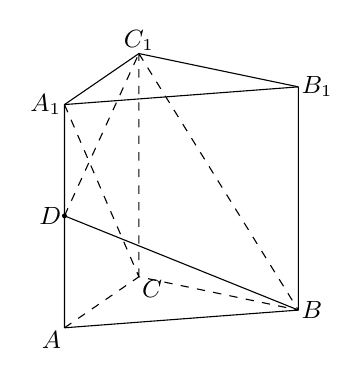
\begin{tikzpicture}[scale=.9, font=\small]
  \coordinate (A)  at (0,0);
  \coordinate (B)  at (3.3,.25);
  \coordinate (C)  at (1.05,.72);
  \coordinate (A1) at (0,3.15);
  \coordinate (B1) at (3.3,3.40);
  \coordinate (C1) at (1.05,3.87);
  \coordinate (D)  at (0,1.58);

  \draw (A)--(B) (A)--(A1) (A1)--(B1) (B)--(B1);
  \draw (A1)--(C1)--(B1);
  \draw (D)--(B);
  \draw[dashed] (A)--(C)--(B) (C)--(C1) (A1)--(C) (C1)--(B);
  \draw[dashed] (D)--(C1);
  \fill (D) circle (1pt);
  \node[below left,inner sep=1pt] at (A) {$A$};
  \node[right,inner sep=1pt] at (B) {$B$};
  \node[below right,inner sep=1pt] at (C) {$C$};
  \node[left,inner sep=1pt] at (A1) {$A_1$};
  \node[right,inner sep=1pt] at (B1) {$B_1$};
  \node[above,inner sep=1pt] at (C1) {$C_1$};
  \node[left,inner sep=1pt] at (D) {$D$};
\end{tikzpicture}
\end{center}
\nopagebreak[4]
（1） 证明：$DC_1\perp BC$；

（2） 求二面角 $A_1-BD-C_1$ 的大小。

\Needspace{4\baselineskip}
\textbf{解析}

\gksubpart{(1) 证明}

\Needspace{5\baselineskip}
设 $AC=BC=a$，则 $AA_1=2a$。取 $C$ 为原点，底面所在平面为 $z=0$，令
\nopagebreak[4]
\[
\overrightarrow{CA}=\boldsymbol u,\qquad
\overrightarrow{CB}=\boldsymbol v,\qquad
|\boldsymbol u|=|\boldsymbol v|=a,
\]
\Needspace{5\baselineskip}
并令竖直单位向量为 $\boldsymbol e$。此时
\nopagebreak[4]
\[
\overrightarrow{DC_1}=a\boldsymbol e-\boldsymbol u,\qquad
\overrightarrow{BD}=\boldsymbol u-\boldsymbol v+a\boldsymbol e.
\]
\Needspace{5\baselineskip}
由题设 $\overrightarrow{DC_1}\perp\overrightarrow{BD}$，得
\nopagebreak[4]
\[
0=(a\boldsymbol e-\boldsymbol u)\cdot
(\boldsymbol u-\boldsymbol v+a\boldsymbol e)
=\boldsymbol u\cdot\boldsymbol v.
\]
\Needspace{5\baselineskip}
所以 $\boldsymbol u\perp\boldsymbol v$，从而
\nopagebreak[4]
\[
\overrightarrow{DC_1}\cdot\overrightarrow{BC}
=(a\boldsymbol e-\boldsymbol u)\cdot\boldsymbol v=0,
\]
即 $DC_1\perp BC$。

\gksubpart{(2) 解}

\Needspace{5\baselineskip}
在上述结论下建立坐标系：
\nopagebreak[4]
\[
\begin{aligned}
C&=(0,0,0),\quad A=(a,0,0),\quad B=(0,a,0),\\
A_1&=(a,0,2a),\quad C_1=(0,0,2a),\quad D=(a,0,a).
\end{aligned}
\]
\Needspace{5\baselineskip}
取平面 $A_1BD$、$C_1BD$ 的法向量
\nopagebreak[4]
\[
\boldsymbol n_1=\overrightarrow{BD}\times\overrightarrow{BA_1}
=a^2(-1,-1,0),
\]
\nopagebreak[4]
\[
\boldsymbol n_2=\overrightarrow{BD}\times\overrightarrow{BC_1}
=a^2(-1,-2,-1).
\]
\Needspace{5\baselineskip}
于是
\nopagebreak[4]
\[
\cos\theta=\frac{\boldsymbol n_1\cdot\boldsymbol n_2}
{|\boldsymbol n_1|\,|\boldsymbol n_2|}
=\frac{3}{\sqrt2\sqrt6}=\frac{\sqrt3}{2},
\]
故二面角 $A_1-BD-C_1$ 的大小为 $30^\circ$。

\gkanswer{答案（1）：见解析版}

\gkanswer{答案（2）：$30^\circ$.}

\end{answer}
\begin{answer}
\gksolhead{20}{}

\textbf{题目}：

设抛物线 $C:x^2=2py$（$p>0$）的焦点为 $F$，准线为 $l$，$A$ 为 $C$ 上一点，已知以 $F$ 为圆心、$FA$ 为半径的圆 $F$ 交 $l$ 于 $B,D$ 两点。

（1） 若 $\angle BFD=90^\circ$，$\triangle ABD$ 的面积为 $4\sqrt2$，求 $p$ 的值及圆 $F$ 的方程；

（2） 若 $A,B,F$ 三点在同一直线 $m$ 上，直线 $n$ 与 $m$ 平行，且 $n$ 与 $C$ 只有一个公共点，求坐标原点到 $m,n$ 距离的比值。

\Needspace{4\baselineskip}
\textbf{解析}

\gksubpart{(1) 解}

\Needspace{5\baselineskip}
焦点为 $F(0,p/2)$，准线为 $y=-p/2$。设圆半径为 $r=FA$。直线 $l$ 到圆心的距离为 $p$，且 $\angle BFD=90^\circ$，所以
\nopagebreak[4]
\[
BD=2\sqrt{r^2-p^2}=r\sqrt2,
\]
\Needspace{5\baselineskip}
从而 $r=p\sqrt2$。由抛物线的焦半径等于点到准线的距离，$A$ 到准线的距离为 $r$。又 $BD=r\sqrt2=2p$，故
\nopagebreak[4]
\[
4\sqrt2=S_{\triangle ABD}
=\frac12\cdot2p\cdot p\sqrt2=p^2\sqrt2,
\]
\Needspace{5\baselineskip}
得到 $p=2$。此时 $F=(0,1)$、$r=2\sqrt2$，圆 $F$ 的方程为
\nopagebreak[4]
\[
x^2+(y-1)^2=8.
\]

\gksubpart{(2) 解}

\Needspace{5\baselineskip}
用参数 $t$ 表示抛物线上的点
\nopagebreak[4]
\[
A=\left(pt,\frac{pt^2}{2}\right),\qquad
F=\left(0,\frac p2\right).
\]
\Needspace{5\baselineskip}
因为 $B$ 在准线上、$A,B,F$ 共线且 $FA=FB$，由同一直线上两段等长可得 $t^2=3$（另一根 $t^2=-1$ 不可取）。取 $t=\sqrt3$，另一侧只改变斜率符号，故
\nopagebreak[4]
\[
m:\ y=\frac{x}{\sqrt3}+\frac p2.
\]
\Needspace{5\baselineskip}
原点到 $m$ 的距离为 $\dfrac{\sqrt3p}{4}$。与 $m$ 平行且与抛物线相切的直线为
\nopagebreak[4]
\[
n:\ y=\frac{x}{\sqrt3}-\frac p6,
\]
原点到 $n$ 的距离为 $\dfrac{\sqrt3p}{12}$，所求比值为 $3:1$。

\gkanswer{答案（1）：$p=2$,圆 $F$ 的方程为 $x^2+(y-1)^2=8$.}

\gkanswer{答案（2）：$3:1$.}

\end{answer}
\begin{answer}
\gksolhead{21}{}

\textbf{题目}：

\Needspace{5\baselineskip}
已知函数 $f(x)$ 满足

\nopagebreak[4]
\[
f(x)=f'(1)\mathrm e^{x-1}-f(0)x+\frac12x^2.
\]

（1） 求 $f(x)$ 的解析式及单调区间；

（2） 若 $f(x)\geqslant\dfrac12x^2+ax+b$，求 $(a+1)b$ 的最大值。

\Needspace{4\baselineskip}
\textbf{解析}

\gksubpart{(1) 解}

\Needspace{5\baselineskip}
令 $A_0=f'(1)$、$B_0=f(0)$。在题设等式中取 $x=0$，得 $B_0=A_0\mathrm e^{-1}$。对等式求导并令 $x=1$，得
\nopagebreak[4]
\[
A_0=A_0-B_0+1,
\]
\Needspace{5\baselineskip}
故 $B_0=1$、$A_0=\mathrm e$。于是
\nopagebreak[4]
\[
f(x)=\mathrm e^x-x+\frac12x^2,
\qquad
f'(x)=\mathrm e^x+x-1.
\]
又 $f''(x)=\mathrm e^x+1>0$，且 $f'(0)=0$，所以 $f(x)$ 在 $(-\infty,0)$ 上单调递减，在 $(0,+\infty)$ 上单调递增。

\gksubpart{(2) 解}

\Needspace{5\baselineskip}
不等式对一切实数 $x$ 成立，当且仅当
\nopagebreak[4]
\[
\mathrm e^x\geqslant (a+1)x+b.
\]
\Needspace{5\baselineskip}
令 $c=a+1$。若 $c<0$，令 $x\to-\infty$ 即矛盾；若 $c=0$，则 $b\leqslant0$，目标值不超过 $0$。当 $c>0$ 时，指数函数在 $x=\ln c$ 处的切线给出且恰为最强条件
\nopagebreak[4]
\[
b\leqslant c(1-\ln c).
\]
\Needspace{5\baselineskip}
因此
\nopagebreak[4]
\[
(a+1)b=cb\leqslant c^2(1-\ln c).
\]
\Needspace{5\baselineskip}
令 $u=\ln c$，则右端为 $\mathrm e^{2u}(1-u)$，其最大值在 $u=\frac12$ 处取得，故
\nopagebreak[4]
\[
c=\sqrt{\mathrm e},\qquad b=\frac{\sqrt{\mathrm e}}2,
\]
最大值为 $\dfrac{\mathrm e}{2}$。

\gkanswer{答案（1）：$f(x)=\mathrm e^x-x+\dfrac12x^2$;在 $(-\infty,0)$ 上单调递减,在 $(0,+\infty)$ 上单调递增.}

\gkanswer{答案（2）：$\dfrac{\mathrm e}{2}$.}

\end{answer}
\begin{answer}
\gksolhead{22}{}

\textbf{题目}：

如图，$D,E$ 分别为 $\triangle ABC$ 边 $AB,AC$ 的中点，直线 $DE$ 交 $\triangle ABC$ 的外接圆于 $F,G$ 两点。若 $CF\parallel AB$，证明：
\nopagebreak[4]
\begin{center}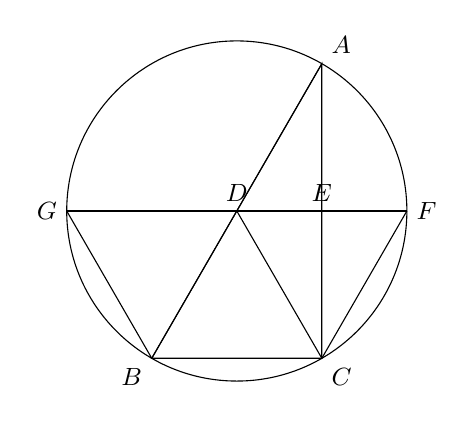
\begin{tikzpicture}[scale=.72, every node/.style={font=\small}]
  \coordinate (G) at (-3,0);
  \coordinate (F) at (3,0);
  \coordinate (A) at (1.5,2.598);
  \coordinate (B) at (-1.5,-2.598);
  \coordinate (C) at (1.5,-2.598);
  \coordinate (D) at (0,0);
  \coordinate (E) at (1.5,0);
  \draw (0,0) circle (3);
  \draw (G)--(F);
  \draw (A)--(B)--(C)--cycle;
  \draw (D)--(C);
  \draw (G)--(B);
  \draw (C)--(F);
  \draw (A)--(C);
  \draw (A)--(B);
  \node[above right] at (A) {$A$};
  \node[below left] at (B) {$B$};
  \node[below right] at (C) {$C$};
  \node[above] at (D) {$D$};
  \node[above] at (E) {$E$};
  \node[left] at (G) {$G$};
  \node[right] at (F) {$F$};
\end{tikzpicture}
\end{center}
\nopagebreak[4]
（1） $CD=BC$；

（2） $\triangle BCD\sim\triangle GBD$。

\Needspace{4\baselineskip}
\textbf{解析}

\gksubpart{(1) 证明}

\Needspace{5\baselineskip}
设 $D=(0,0)$，取 $A=(-1,0)$、$B=(1,0)$、$C=(u,v)$，其中 $v\ne0$。则
\nopagebreak[4]
\[
E=\left(\frac{u-1}{2},\frac v2\right),
\]
\Needspace{5\baselineskip}
直线 $DE$ 的方向向量为 $(u-1,v)$。由 $CF\parallel AB$，且 $F$ 在直线 $DE$ 上，得
\nopagebreak[4]
\[
F=(u-1,v).
\]
\Needspace{5\baselineskip}
过 $A,B,C$ 的圆方程可写为
\nopagebreak[4]
\[
x^2+y^2+\lambda y=1.
\]
\Needspace{5\baselineskip}
把 $C$ 和 $F$ 代入圆方程并相减，得到 $u=\frac12$。于是
\nopagebreak[4]
\[
CD^2=\frac14+v^2=BC^2,
\]
故 $CD=BC$。

\gksubpart{(2) 证明}

\Needspace{5\baselineskip}
记 $s=\frac14+v^2$。直线 $DE$ 可参数化为
\nopagebreak[4]
\[
(x,y)=\left(-\frac t2,tv\right).
\]
\Needspace{5\baselineskip}
代入外接圆方程，两个交点对应的参数为 $t=1$（点 $F$）和 $t=-1/s$（点 $G$）。因而
\nopagebreak[4]
\[
G=\left(\frac1{2s},-\frac v s\right).
\]
\Needspace{5\baselineskip}
直接计算得
\nopagebreak[4]
\[
BC=CD=\sqrt s,\qquad BG=BD=1,\qquad GD=\frac1{\sqrt s}.
\]
\Needspace{5\baselineskip}
所以
\nopagebreak[4]
\[
\frac{BC}{BG}=\frac{CD}{BD}=\frac{BD}{GD}=\sqrt s,
\]
\Needspace{5\baselineskip}
由三边对应成比例，得
\nopagebreak[4]
\[
\triangle BCD\sim\triangle GBD.
\]

\gkanswer{答案（1）：见解析版}

\gkanswer{答案（2）：见解析版}

\end{answer}
\begin{answer}
\gksolhead{23}{}

\textbf{题目}：

\Needspace{5\baselineskip}
已知曲线 $C_1$ 的参数方程是

\nopagebreak[4]
\[
\begin{cases}
x=2\cos\varphi,\\
y=3\sin\varphi,
\end{cases}
\qquad(\varphi\text{ \text{是参数}}).
\]

以坐标原点为极点，$x$ 轴的非负半轴为极轴建立极坐标系，曲线 $C_2$ 的极坐标方程是 $\rho=2$，正方形 $ABCD$ 的顶点都在 $C_2$ 上，且 $A,B,C,D$ 依逆时针次序排列，点 $A$ 的极坐标为 $\left(2,\dfrac{\pi}{3}\right)$。

（1） 求点 $A,B,C,D$ 的直角坐标；

（2） 设 $P$ 为 $C_1$ 上任意一点，求 $|PA|^2+|PB|^2+|PC|^2+|PD|^2$ 的取值范围。

\Needspace{4\baselineskip}
\textbf{解析}

\gksubpart{(1) 解}

\Needspace{5\baselineskip}
正方形外接圆半径为 $2$，相邻顶点的极角相差 $\frac\pi2$。依逆时针次序，四点极角为
\nopagebreak[4]
\[
\frac\pi3,\quad\frac{5\pi}6,\quad\frac{4\pi}3,\quad\frac{11\pi}6.
\]
\Needspace{5\baselineskip}
所以
\nopagebreak[4]
\[
A=(1,\sqrt3),\quad B=(-\sqrt3,1),\quad C=(-1,-\sqrt3),\quad D=(\sqrt3,-1).
\]

\gksubpart{(2) 解}

\Needspace{5\baselineskip}
设 $P=(x,y)$。正方形四个顶点的坐标和为零，且每个顶点到原点的距离平方为 $4$，故
\nopagebreak[4]
\[
\begin{aligned}
&|PA|^2+|PB|^2+|PC|^2+|PD|^2\\
&=4(x^2+y^2)+16.
\end{aligned}
\]
\Needspace{5\baselineskip}
由参数方程 $x=2\cos\varphi$、$y=3\sin\varphi$，有
\nopagebreak[4]
\[
4(x^2+y^2)+16=16\cos^2\varphi+36\sin^2\varphi+16.
\]
故取值范围为 $[32,52]$。

\gkanswer{答案（1）：$A(1,\sqrt3)$,$B(-\sqrt3,1)$,$C(-1,-\sqrt3)$,$D(\sqrt3,-1)$.}

\gkanswer{答案（2）：$[32,52]$.}

\end{answer}
\begin{answer}
\gksolhead{24}{}

\textbf{题目}：

已知函数 $f(x)=|x+a|+|x-2|$。

（1） 当 $a=-3$ 时，求不等式 $f(x)\geqslant3$ 的解集；

（2） 若 $f(x)\leqslant|x-4|$ 的解集包含 $[1,2]$，求 $a$ 的取值范围。

\Needspace{4\baselineskip}
\textbf{解析}

\gksubpart{(1) 解}

\Needspace{5\baselineskip}
当 $a=-3$ 时，$f(x)=|x-3|+|x-2|$。分三段讨论：
\nopagebreak[4]
\[
x\leqslant2:\quad 5-2x\geqslant3\Longleftrightarrow x\leqslant1;
\]
\nopagebreak[4]
\[
2\leqslant x\leqslant3:\quad 1\geqslant3\quad\text{无解};
\]
\nopagebreak[4]
\[
x\geqslant3:\quad 2x-5\geqslant3\Longleftrightarrow x\geqslant4.
\]
所以解集为 $(-\infty,1]\cup[4,+\infty)$。

\gksubpart{(2) 解}

\Needspace{5\baselineskip}
对 $x\in[1,2]$，有 $|x-2|=2-x$、$|x-4|=4-x$，原不等式等价于
\nopagebreak[4]
\[
|x+a|\leqslant2.
\]
\Needspace{5\baselineskip}
要对整个区间 $[1,2]$ 成立，必须且只需
\nopagebreak[4]
\[
1+a\geqslant-2,\qquad 2+a\leqslant2,
\]
\Needspace{5\baselineskip}
即
\nopagebreak[4]
\[
-3\leqslant a\leqslant0.
\]

\gkanswer{答案（1）：$(-\infty,1]\cup[4,+\infty)$.}

\gkanswer{答案（2）：见解析版}

\end{answer}